\section{The clock as a random variable}\label{ch:clocklaw}

The clock variable $T$ of Section~\ref{ch:clock}, with $\E e^{-uT}=1/G(u)$, exists unconditionally and is self decomposable (Theorem~\ref{thm:ch12:idsd}). Under RH it is $T=\sum_{\gamma>0}e_\gamma/\gamma^2$ with independent standard exponential variables $e_\gamma$ (Proposition~\ref{prop:rigid}), and if the zeros are also simple, the theorems of Kent and Krein make it the hitting time of a level by a diffusion whose Dirichlet spectrum is $\{\gamma^2\}$ \cite{Kent80}, \cite[Section 16.3]{P26}. Its law can be computed from the P\'olya density with no zero as input, and the first zero appears in it as the rate of decay, $\gamma_1^2$ (Section~\ref{sec:ch18:law}). The other zeros are much harder to see: in time they enter through exponentially subdominant terms that cost digits of accuracy, and Monte Carlo sampling through Williams' representation of the P\'olya variable needs about $10^6$ draws to show even the first zero (Section~\ref{sec:ch18:reach}). Computation can instead approximate the clock by explicit generalised gamma convolutions that keep the verified zeros as atoms and replace the others by a smooth tail (Section~\ref{sec:ch18:kent}); at large values of the variable $u$ their error is governed by the argument function $S(t)$ beyond the last zero used (Section~\ref{sec:ch18:moments}).

\subsection{The law of the clock and its decay rate}\label{sec:ch18:law}

The Laplace transform $\E e^{-uT}=\xi(\tfrac12)/\xi(\tfrac12+\sqrt u)$ is available from the P\'olya route at every complex $u$ other than its poles, untilted for $|\im\sqrt u|<120$ and tilted above (Section~\ref{sec:newcomp}). Talbot's contour inversion \cite{Talbot79}, as implemented in \texttt{mpmath} \cite{mpmath}, then gives the density $f$ of $T$ and its survival function $\bar F(t)=P(T>t)$ with no reference to the zeros.

Under RH, with simple zeros, the density also has the spectral expansion \cite{Kent80}
\[
f(t)=\sum_k R_ke^{-\gamma_k^2t},\qquad P(T>t)=\sum_k\frac{R_k}{\gamma_k^2}e^{-\gamma_k^2t},\qquad R_k=\frac{2i\gamma_k\,\xi(\tfrac12)}{\xi'(\tfrac12+i\gamma_k)},
\]
whose coefficients are the residues of the transform at its poles $u=-\gamma_k^2$. The first step of the proof of Theorem~\ref{bs:thm:nb} derives it by a contour shift, with $R_k=-2\gamma_k\Xi(0)/\Xi'(\gamma_k)$ in the role of $c_n$ there, and the P\'olya route supplies both the ordinates, as its Newton roots, and the values of $\xi'$ at them. The residues alternate in sign, because $\Xi'$ changes sign at consecutive simple zeros (Exercise~\ref{ex:ch18:residues}), and they grow like $e^{\pi\gamma_k/4}$ up to powers of $\gamma_k$ and the factor $1/|\zeta'(\rho_k)|$, because Stirling's formula puts the factor $e^{-\pi\gamma_k/4}$ into $|\Xi'(\gamma_k)|=|\xi'(\rho_k)|$; thus $R_1=1.0164\times10^4$ and $R_2=-1.1775\times10^6$. The series converges for $t>0$ but cancels heavily at small $t$, so near the origin Talbot's contour, which uses the transform only away from the poles, is the better tool (Exercise~\ref{ex:ch18:origin}); under the hypotheses of Theorem~\ref{bs:thm:nb} the line $\re t=0$ is a natural boundary of the density. Computed with $50$ digits from the $79$ zeros below $200$, the spectral expansion agrees with the Talbot values to $24$ digits for $0.010\le t\le0.12$. Beyond that range the Talbot values lose relative accuracy as $\bar F(t)$ falls, down to six digits at $t=0.3$, and the spectral expansion is the accurate one (Figure~\ref{fig:clocklaw}).

The law is unimodal with no hypothesis (Corollary~\ref{sb:cor:unimodal}) and sharply concentrated. Its mean and variance are $\E T=0.0231050$ and $\operatorname{Var}T=3.71726\times10^{-5}$ (Section~\ref{ch:clock}) and its median is $0.0220$; $P(T\le0.009)=1.4\times10^{-7}$, the density is $6.5\times10^{-24}$ at $t=0.005$, and $P(T>0.1)=1.07\times10^{-7}$.

The hazard $h=f/\bar F$ tends to the principal eigenvalue $\gamma_1^2$. Under RH with simple zeros the leading term of the spectral expansion dominates, and $h(t)-\gamma_1^2=O(e^{-(\gamma_2^2-\gamma_1^2)t})$ (Exercise~\ref{ex:ch18:hazard}). This is the quasi stationary behaviour of a hitting time; Roberts \cite[Section 2]{Roberts91} obtains approximations of Brownian boundary hitting laws from approximations of the conditioned diffusion. The Talbot side shows the limit with no zero as input: $h(0.05)=199.72$, $h(0.1)=199.7904544$ and $h(0.25)=199.79045483$, the last equal to $\gamma_1^2$ to the eleven digits shown, which is the accuracy of the inversion that far into the tail. The spectral expansion, which has $\gamma_1$ as input, gives $h(0.25)=199.790454832386859463$, equal to $\gamma_1^2$ to all $21$ digits. The rate of approach is the spectral gap: a fit of $\log|h(t)-\gamma_1^2|$ on $[0.05,0.12]$ has slope $-242.12$, against $-(\gamma_2^2-\gamma_1^2)=-242.14$.

\begin{figure}[t]
\centering
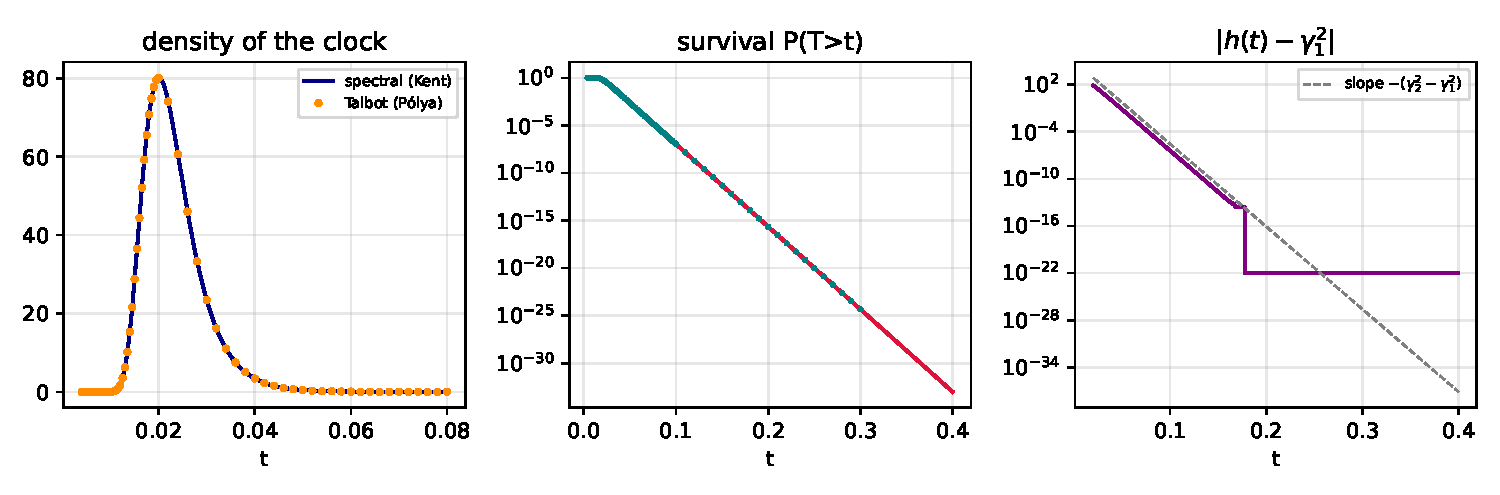
\includegraphics[width=\textwidth]{fig/clocklaw.pdf}
\caption{The law of the clock variable computed from the P\'olya density by Talbot inversion (points) and by the spectral expansion with P\'olya residues (lines): density, survival function, and the distance of the hazard from $\gamma_1^2$, whose logarithm has slope $-(\gamma_2^2-\gamma_1^2)$ (dashed). Beyond $t\approx0.17$ the last curve reflects the double precision of the plotting script, not the hazard.}
\label{fig:clocklaw}
\end{figure}

\subsection{The cost of the zeros in time and in samples}\label{sec:ch18:reach}

The time domain sees the higher atoms only through exponentially subdominant terms. We fit sums of $p$ exponentials to $P(T>t)$ by Prony's method, from $40$ values at $t=0.03,0.032,\dots,0.108$ carrying relative noise from $10^{-16}$ down to $10^{-45}$ (Table~\ref{tab:prony}). With $p=4$ terms the first atom is correct to all nine digits shown, the second to six, the third to four and the fourth to two per cent, and the results do not improve as the noise falls. The error comes from the neglected terms, whose relative size on a window starting at $t_0$ is $e^{-(\gamma_{p+1}^2-\gamma_1^2)t_0}$ up to a factor set by the residues. Resolving the $k$th atom therefore needs data accurate to about $(\gamma_k^2-\gamma_1^2)t_0/\log10$ digits, a number that grows without bound in $k$: a hazard rate method reaches the first atom, and every further atom costs digits.

\begin{table}[t]
\centering\small
\begin{tabular}{rllll}
\toprule
terms & $\gamma_1^2$ & $\gamma_2^2$ & $\gamma_3^2$ & $\gamma_4^2$\\
\midrule
2 & 199.86679 & 427.28 & & \\
3 & 199.79031 & 442.129 & 618.93 & \\
4 & 199.790455 & 441.9255 & 625.63 & 907.24\\
\midrule
true & 199.7904548 & 441.9261506 & 625.5429969 & 925.6730873\\
\bottomrule
\end{tabular}
\caption{Prony extraction of the atoms from $P(T>t)$ on $t\in[0.03,0.108]$. Identical results for relative noise $10^{-16}$, $10^{-30}$ and $10^{-45}$: the error is model truncation, not noise.}
\label{tab:prony}
\end{table}

Sampling meets the same cancellation in another currency. By the identity $2\xi(s)=\E[(\pi S_2/2)^{s/2}]$ of Section~\ref{ch:clock}, with $S_2=\sum_{k\ge1}\frac2{\pi^2k^2}\Gamma_k$ for independent Gamma$(2,1)$ variables $\Gamma_k$, the variable $Y=\frac12\log(\pi S_2/2)$ satisfies
\[
2\,\Xi(z)=\E\big[e^{Y/2}\cos(zY)\big].
\]
The P\'olya variable is $Y$ tilted by $e^{Y/2}$, and $\Xi(z)$ is the mean of a random variable with finite variance, since $\E e^{Y}=2\xi(1)=1$, so a sample mean estimates it at every $z$. We draw $n=10^6$ copies of $S_2$, truncating the series after $2000$ terms and replacing the remainder, whose variance is about $3\times10^{-12}$, by its mean $4/(2000\pi^2)$, and compare the estimates with $\Xi(z)$ in Table~\ref{tab:ch18:mc}, a check of the identity on the critical line; Table~\ref{bp:tab:bpy} checks it at real $s$ (Section~\ref{bp:sec:mellin}).

\begin{table}[htbp]
\centering\small
\begin{tabular}{rllll}
\toprule
$z$ & Monte Carlo & standard error & $\Xi(z)$ & $n$ with standard error $|\Xi(z)|$\\
\midrule
0 & 0.497061 & $5.4\times10^{-5}$ & 0.497121 & $1.2\times10^{-2}$\\
2 & 0.453136 & $7.3\times10^{-5}$ & 0.453100 & $2.6\times10^{-2}$\\
5 & 0.275888 & $2.4\times10^{-4}$ & 0.275550 & $0.77$\\
8 & 0.103756 & $3.4\times10^{-4}$ & 0.103303 & $11$\\
10 & 0.038401 & $3.5\times10^{-4}$ & 0.037968 & $86$\\
20 & 0.000314 & $3.5\times10^{-4}$ & $-3.67\times10^{-5}$ & $9.3\times10^{7}$\\
30 & 0.000289 & $3.5\times10^{-4}$ & $-1.50\times10^{-8}$ & $5.5\times10^{14}$\\
\bottomrule
\end{tabular}
\caption{Monte Carlo estimates of $\Xi(z)$ from Williams' representation with $10^6$ samples. The last column is the sample size at which the standard error equals $|\Xi(z)|$.}
\label{tab:ch18:mc}
\end{table}

The standard error settles at $3.5\times10^{-4}$, the standard deviation of $e^{Y/2}\cos(zY)/2$ over $\sqrt n$, while $|\Xi(z)|$ decays like $e^{-\pi z/4}$. The sample size needed to resolve the sign of $\Xi$ therefore grows like $e^{\pi z/2}$: about $10^8$ at $z=20$ and $10^{15}$ at $z=30$. Even the first sign change, at $z=14.13$, needs about $10^{6}$ samples: between the first two zeros $|\Xi|$ is at most $8.0\times10^{-4}$ (at $z=15.59$), and resolving it at two standard errors takes about $8\times10^5$ samples. Figure~\ref{fig:ch18:mc} shows where $|\Xi|$ falls below the standard error. The P\'olya route pays for the same cancellation in digits of working precision and Monte Carlo pays for it in samples, and precision is exponentially cheaper. Sampling is the right tool for the law of the P\'olya variable itself, for its moments and for the Bayesian inverse problems of \cite[Section 19.2]{P26}, and the wrong tool for the zeros. Devroye's exact samplers for theta type laws \cite{Devroye86} make sampling efficient, but the sample size needed for the zeros still grows like $e^{\pi z/2}$.

\begin{figure}[!ht]
\centering
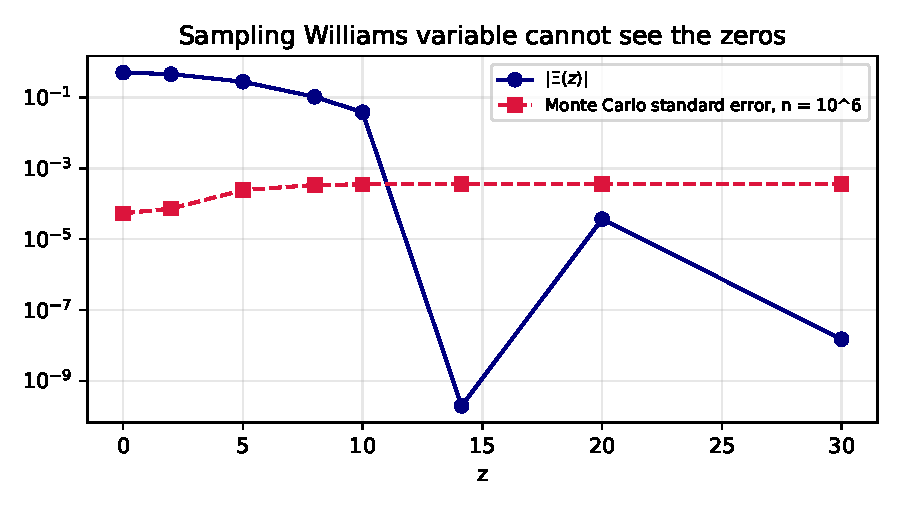
\includegraphics[width=0.72\textwidth]{fig/williams_mc.pdf}
\caption{$|\Xi(z)|$ against the Monte Carlo standard error with $10^6$ samples of Williams' variable $S_2$, at the sampled values of $z$ and at the first zero, joined by straight lines.}
\label{fig:ch18:mc}
\end{figure}

\subsection{Kent approximants with a Weyl tail}\label{sec:ch18:kent}

In the rest of this section we write $w$ for the variable $u$ of the clock, as the tables and figures that follow do. Kent's theorem \cite{Kent80} identifies the first hitting time of a level by a diffusion started at a reflecting or entrance end of its interval with the GGC $\prod_n(1+w/\lambda_n)^{-1}$, where the $\lambda_n$ are the Dirichlet eigenvalues of the interval up to that level; the simplest example is the time a three dimensional Bessel process started at $0$ takes to reach the level one, with $\lambda_n=\pi^2n^2/2$ (Section~\ref{bp:sec:mellin}). Krein's inverse spectral theory \cite{DymMcKean76} builds a string, and so a generalised diffusion, from any increasing sequence $\lambda_n>0$ with $\sum1/\lambda_n<\infty$. The GGCs that arise as such hitting times are therefore exactly those without drift whose Thorin measure consists of unit atoms at distinct points. By Proposition~\ref{prop:rigid} the clock is one of them exactly when RH holds and the zeros are simple, and its diffusion then has Dirichlet spectrum $\{\gamma^2\}$; Section~\ref{ri:sec:kill} reads each $1/\zeta(2k)$, up to an explicit factor, as the probability that this diffusion reaches its level before an independent killing. The shifted clocks above the centre are not hitting times of Kent's kind, but with no hypothesis they are the tilted centre clock run through the inverse local time of a sticky Brownian motion (Section~\ref{ch:bphit}), and Section~\ref{pm:sec:map} places all these processes in one map.

The approximants of the clock that Kent's theorem suggests are the transforms $1/G_N(w)$ of the partial products $G_N(w)=\prod_{k\le N}(1+w/\gamma_k^2)$, each the transform of the hitting time of a finite string with $N$ point masses. They are admissible in the closure criterion of Corollary~\ref{cor:weak:closure}, and they are the approximating sequence, under RH, in the proof of \cite[Proposition 18.10]{P26}; Section~\ref{sec:weak:limits} lists them, with and without the Weyl tail of this section, among the approximants whose positivity is proved independently of $\xi$. They converge slowly. With $\tau_1(N)=\sum_{k>N}\gamma_k^{-2}$, the relative error $G(w)/G_N(w)-1$ of the clock transform lies, under RH, between $w\tau_1(N)$ and $e^{w\tau_1(N)}-1$; it is of order one at $w=100$ for $N=20$ and at $w=1000$ for $N=300$.

We keep the verified zeros as atoms and replace the others by their average density. By the Riemann von Mangoldt formula $N(t)=\vartheta(t)/\pi+1+S(t)$, with the Riemann Siegel theta function $\vartheta$ and the argument function $S(t)=\pi^{-1}\arg\zeta(\frac12+it)$ of Section~\ref{ch:classical}, the zeros above the cutoff $\Theta_N$ have density $\vartheta'(\gamma)/\pi\approx\frac1{2\pi}\log\frac\gamma{2\pi}$, which is positive for $\gamma>6.3$. So
\[
G_N^{\rm W}(w)=\prod_{k\le N}\Big(1+\frac w{\gamma_k^2}\Big)\exp\Big\{\int_{\Theta_N}^\infty\log\Big(1+\frac w{\gamma^2}\Big)\frac{\vartheta'(\gamma)}\pi\,d\gamma\Big\},
\]
with W for Weyl, has reciprocal equal to the Laplace transform of a GGC with $N$ unit atoms and the continuous Thorin density $\vartheta'(\sqrt z)/(2\pi\sqrt z)$ on $z>\Theta_N^2$. That Thorin measure is not a sum of unit atoms, so, unlike $1/G_N$, the approximant is not a hitting time of the kind in Kent's theorem; the closure criterion needs only the GGC property. For $\Theta_N$ we take the Gram point $g_{N-1}$ of Section~\ref{sec:ch5:turing}, where $\vartheta(\Theta_N)/\pi+1=N$. For the values of $N$ used here it lies between $\gamma_N$ and $\gamma_{N+1}$, so $S(\Theta_N)=0$ and the smooth count agrees with the true count at the cutoff, as in Section~\ref{ch:distances}, where $\Theta_{1700}$ is the point $T_*$.

Table~\ref{tab:ch18:kent} compares the two approximants with the clock computed from $\xi$. The Weyl tail improves the approximation by at least two orders of magnitude at every $N$ and $w$ tested. With the first $1700$ zeros ($\gamma_{1700}=2197.26$) its error is $3\times10^{-11}$ at $w=1$ and $3\times10^{-7}$ at $w=10^4$, where the partial product is wrong by a factor of more than a hundred. Figure~\ref{fig:ch18:kent} plots the same data.

\begin{table}[htbp]
\centering\footnotesize
\setlength{\tabcolsep}{4pt}
\begin{tabular}{rllll}
\toprule
$N$ & $w=1$ & $w=100$ & $w=1000$ & $w=10^4$\\
\midrule
1 & $1.8\times10^{-2}$ / $1.3\times10^{-4}$ & $4.8$ / $1.0\times10^{-2}$ & $\gg1$ / $3.3\times10^{-2}$ & $\gg1$ / $4.3\times10^{-2}$\\
20 & $7.2\times10^{-3}$ / $4.3\times10^{-7}$ & $1.04$ / $4.2\times10^{-5}$ & $\gg1$ / $3.7\times10^{-4}$ & $\gg1$ / $1.5\times10^{-3}$\\
79 & $3.6\times10^{-3}$ / $1.5\times10^{-7}$ & $0.43$ / $1.5\times10^{-5}$ & $34$ / $1.5\times10^{-4}$ & $\gg1$ / $1.2\times10^{-3}$\\
300 & $1.6\times10^{-3}$ / $7.4\times10^{-9}$ & $0.17$ / $7.4\times10^{-7}$ & $3.95$ / $7.4\times10^{-6}$ & $\gg1$ / $7.2\times10^{-5}$\\
1700 & $5.0\times10^{-4}$ / $2.9\times10^{-11}$ & $0.051$ / $2.9\times10^{-9}$ & $0.64$ / $2.9\times10^{-8}$ & $142$ / $2.9\times10^{-7}$\\
\bottomrule
\end{tabular}
\caption{Relative error of the clock transform: partial product over $N$ zeros, $|G/G_N-1|$, and with the Weyl tail, $|G_N^{\rm W}/G-1|$. The two measures of error agree to first order, and $\gg1$ marks an error above $10^3$. The partial product values agree with \cite[Section 18.2.1]{P26} where both are given.}
\label{tab:ch18:kent}
\end{table}

\begin{figure}[htbp]
\centering
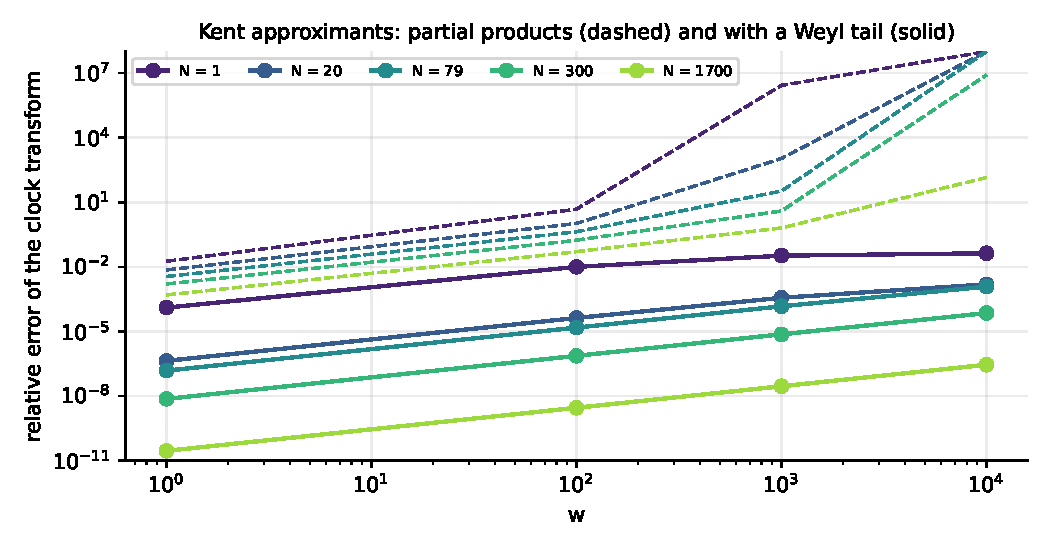
\includegraphics[width=0.8\textwidth]{fig/kenttail.pdf}
\caption{Relative error of Kent approximants to the clock transform, without (dashed) and with (solid) the Weyl tail.}
\label{fig:ch18:kent}
\end{figure}

At the four points $w=1,100,1000,10^4$ the table exhibits an explicit positive Thorin measure whose Thorin transform $\int\log(1+w/z)\,U(dz)$ matches $\log G(w)$ to within $3\times10^{-7}$. This is a finite instance of the weak Thorin condition of \cite[Section 18.2.3]{P26}, which asks for such a measure, to within any $\eta>0$, at every finite set of points, and which is equivalent to RH by the closure criterion of Corollary~\ref{cor:weak:closure}. A finite instance proves nothing: agreement for $w\le10^4$ cannot detect off line zeros above the verified height, which change $\log G$ there by far less than the error. The error of the Weyl tail grows linearly in $w$, and to first order it is a weighted average of $S$ beyond the cutoff,
\[
\log G(w)-\log G_N^{\rm W}(w)\approx w\big(\tau_1(N)-\tau_1^{\rm W}(N)\big)=2w\int_{\Theta_N}^\infty\frac{S(\gamma)}{\gamma^3}\,d\gamma,
\]
where $\tau_1^{\rm W}(N)=\int_{\Theta_N}^\infty\gamma^{-2}\vartheta'(\gamma)\pi^{-1}d\gamma$ is the Weyl estimate of $\tau_1(N)$ and the identity is an integration by parts that uses $S(\Theta_N)=0$. No tail built on the smooth count can follow $S$ without the zeros. The Taylor coefficients of $\xi$ at the centre carry more information, and Section~\ref{sec:ch18:moments} uses them.

\subsection{Moment matching and the error at large $w$}\label{sec:ch18:moments}

The error of the Weyl tail comes from the first order term of $\log(1+w/\gamma^2)=w/\gamma^2-w^2/(2\gamma^4)+\cdots$. For $w$ small compared with $\Theta_N^2$ the error of $\log G_N^{\rm W}$ is approximately $w$ times $\tau_1(N)-\tau_1^{\rm W}(N)$, and the second order term is $-w^2/2$ times the corresponding difference for $\tau_2(N)=\sum_{k>N}\gamma_k^{-4}$. Both true tail sums are available without any zero beyond $\gamma_N$, because the power sums $p_m=\sum_ka_k^{-m}$, with $a_k=-(\rho_k-\frac12)^2$ as in Section~\ref{ch:clock} and equal to $\sum_{\gamma>0}\gamma^{-2m}$ under RH, are Taylor coefficients of $\xi$ at the centre: if $\xi(\frac12+s)/\xi(\frac12)=1+c_2s^2+c_4s^4+\cdots$, then
\begin{gather*}
p_1=\sum_ka_k^{-1}=c_2=0.0231049931154189707889,\\
p_2=\sum_ka_k^{-2}=c_2^2-2c_4=0.0000371725992852696862,
\end{gather*}
and $\tau_m(N)=p_m-\sum_{k\le N}\gamma_k^{-2m}$. Here $p_1=\E T$ and $p_2=\operatorname{Var}T$ (Section~\ref{ch:clock}). We therefore replace the Weyl density $\vartheta'(\gamma)/\pi$ on $[\Theta_N,\infty)$ by $\lambda\,\vartheta'(\gamma)/\pi$ on $[\Theta_N',\infty)$, and choose the two parameters $\lambda$ and $\Theta_N'$ so that the tail reproduces $\tau_1(N)$ and $\tau_2(N)$ exactly. The tail density remains positive, so the approximant is still a GGC. The adjustments are small: for $N=79$ the cutoff moves from $199.649$ to $199.675$ and $\lambda=1.000059$, and for $N=1700$ it moves from $2197.87959$ to $2197.87923$ and $\lambda=0.99999992$.

\begin{table}[htbp]
\centering\footnotesize
\setlength{\tabcolsep}{4pt}
\begin{tabular}{rlllllll}
\toprule
$N$ & tail & $w=1$ & $w=10^2$ & $w=10^4$ & $w=10^5$ & $w=10^6$ & $w=10^7$\\
\midrule
79 & Weyl & $1.5\times10^{-7}$ & $1.5\times10^{-5}$ & $1.2\times10^{-3}$ & $4.3\times10^{-3}$ & $5.8\times10^{-3}$ & $6.0\times10^{-3}$\\
 & matched & $2.6\times10^{-17}$ & $2.6\times10^{-11}$ & $1.8\times10^{-5}$ & $3.1\times10^{-3}$ & $6.1\times10^{-2}$ & $0.47$\\
\addlinespace
300 & Weyl & $7.4\times10^{-9}$ & $7.4\times10^{-7}$ & $7.2\times10^{-5}$ & $5.5\times10^{-4}$ & $1.7\times10^{-3}$ & $2.1\times10^{-3}$\\
 & matched & $2.3\times10^{-20}$ & $2.3\times10^{-14}$ & $2.2\times10^{-8}$ & $1.5\times10^{-5}$ & $1.8\times10^{-3}$ & $2.8\times10^{-2}$\\
\addlinespace
1700 & Weyl & $2.9\times10^{-11}$ & $2.9\times10^{-9}$ & $2.9\times10^{-7}$ & $2.8\times10^{-6}$ & $2.4\times10^{-5}$ & $9.3\times10^{-5}$\\
 & matched & $3.5\times10^{-23}$ & $1.1\times10^{-17}$ & $7.0\times10^{-13}$ & $3.6\times10^{-10}$ & $2.5\times10^{-7}$ & $5.0\times10^{-5}$\\
\bottomrule
\end{tabular}
\caption{Relative error $|G_{\rm a}/G-1|$ of the approximant $G_{\rm a}$ of $G$ with the Weyl tail and with the moment matched tail. The cutoffs are $\Theta_N^2=3.99\times10^4$, $2.95\times10^5$ and $4.83\times10^6$ for $N=79$, $300$ and $1700$.}
\label{tab:ch18:kent2}
\end{table}

\begin{figure}[htbp]
\centering
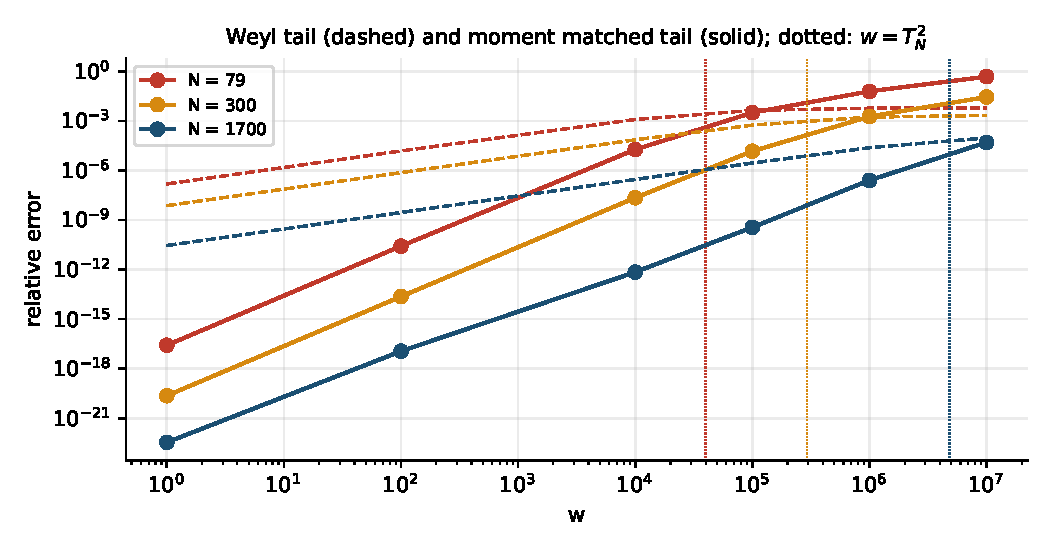
\includegraphics[width=0.8\textwidth]{fig/kenttail2.pdf}
\caption{The Kent approximants at large $w$, with the dotted lines at $w=\Theta_N^2$ (labelled $T_N^2$ in the plot). Moment matching gains ten to twelve digits at $w=1$ and about two as $w$ approaches $\Theta_N^2$. Beyond $\Theta_N^2$ the Weyl tail levels off at a floor set by $S$, while the error of the matched tail, whose density is rescaled by $\lambda$, grows like $|\lambda-1|\sqrt w\log w$.}
\label{fig:ch18:kent2}
\end{figure}

Table~\ref{tab:ch18:kent2} and Figure~\ref{fig:ch18:kent2} show two regimes. For $w$ below $\Theta_N^2$ moment matching gains ten to twelve digits at $w=1$ and about two as $w$ approaches $\Theta_N^2$: with $1700$ zeros the error at $w=10^4$ falls from $2.9\times10^{-7}$ to $7\times10^{-13}$, and at $w=10^5$ from $2.8\times10^{-6}$ to $3.6\times10^{-10}$. Well beyond $\Theta_N^2$ the gain disappears, and at $w=10^7$ with $N=79$ the matched tail is worse than the plain Weyl tail. The cause is the rescaling of the whole tail. For $w\gg\Theta_N^2$ the matched tail differs from the Weyl tail mainly by $(\lambda-1)\int_{\Theta_N'}^\infty\log(1+w/\gamma^2)\,\vartheta'(\gamma)\pi^{-1}d\gamma$, which grows like $(\lambda-1)\frac{\sqrt w}2\log\frac{\sqrt w}{2\pi}$, while the error of the Weyl tail tends to a constant.

That constant is a weighted average of $S$ beyond the cutoff. Under RH, since $S(\Theta_N)=0$ and no ordinate lies in $(\gamma_N,\Theta_N]$, the true tail sum minus its Weyl estimate is a Stieltjes integral against $S$, and an integration by parts gives
\begin{align*}
\log G_N^{\rm W}(w)-\log G(w)&=-\int_{\Theta_N}^\infty\log\Big(1+\frac w{\gamma^2}\Big)\,dS(\gamma)=-\int_{\Theta_N}^\infty\frac{2w\,S(\gamma)}{\gamma(\gamma^2+w)}\,d\gamma\\
&\longrightarrow\;-2\int_{\Theta_N}^\infty\frac{S(\gamma)}\gamma\,d\gamma\qquad(w\to\infty).
\end{align*}
The limit is $-\ell_N$, with $\ell_N=2\int_{\Theta_N}^\infty S(\gamma)\gamma^{-1}\,d\gamma$ as in Exercise~\ref{ex:ch18:floor}. It is finite because $\int_0^tS(u)\,du=O(\log t)$ (Littlewood; Section~\ref{sec:ch5:turing}), and in general it is not zero. The measured errors of the Weyl tail level off at about $6\times10^{-3}$ for $N=79$ and $2\times10^{-3}$ for $N=300$; for $N=1700$ the error is still rising at $w=10^7$, where it is $9.3\times10^{-5}$, so its level is not yet reached.

The constant is not an obstruction of principle. It depends only on $\gamma_1,\dots,\gamma_N$ and on $\xi$ along the real axis, and Stirling's formula gives $\ell_N$ in closed form (Exercise~\ref{ex:ch18:floor}). It is also a floor only for the Weyl density. Adding to $\vartheta'/\pi$ a continuous $\omega$ with compact support in $(\Theta_N,\infty)$ and $\int\omega=0$ changes the limit by $-2\int\omega(\gamma)\log\gamma\,d\gamma$, and two wide bumps of opposite sign placed far apart give this any value while the density stays positive, so a suitable positive tail removes the constant.

Of the two tails computed here, the matched tail is the better one for $w$ up to about $\Theta_N^2$ and the plain Weyl tail beyond. With them the clock is within a small computed distance of an explicit GGC at every scale computed, and at large $w$ that distance is a weighted integral of $S$ beyond the cutoff, the quantity whose integrals Turing's method bounds (Section~\ref{ch:turing}).
